\section{Implementation}
\subsection{Framework}
The implementation was completed in Rust. For the sake of brevity I will not go into depth on why Rust is awesome, you are just going to have to trust me. There are three crucial parts that need to be looked at in our custom filesystem framework:

\begin{itemize}
    \item password hashing
    \item symmetric encryption
    \item asymmetric encryption
\end{itemize}

\subsubsection{Password hashing}

As explained above, the master key is derived from the password. This process uses Argon2\cite{argon2} as a key derivation function. The hashing method is implemented in the cryptography module, it is called the \lstinline{hash_password()} function\cite{hashpass}.

This function is used for two purposes: the first hashing to get the hash of the password (with a server-side stored salt that was initially provided) and then a second hashing to get the challenge hash. When a user is added, he creates a password, this password is hashed without providing a salt, this will generate a random salt. This salt is the one used each time to create the password hash, also known as the master key. 

I am using the \lstinline{argon2} crate\cite{argon2docs}.

\subsubsection{Symmetric encryption}
Symmetric encryption is handled by two functions inside the cryptography module. One to encrypt and the other to decrypt. The algorithm used is AES GCM 256. From the table seen in class the 256 bits key size should be good long term. To encrypt a folder or file, we call this function.

I am using the \lstinline{aes_gcm} crate\cite{aesgcm}.

\subsubsection{Asymmetric encryption}
Asymmetric encryption is necessary for signing and sharing capabilities. This is why the user structure has two key pairs, one to sign with, the other to encrypt with. This was specifically advised by the crate used for signing \lstinline{dryoc}: "One should take note that keys used for signing and encryption should remain separate. While it’s possible to convert Ed25519 keys to X25519 keys (or derive them from the same seed), one is cautioned against doing so."\cite{dryocsign}

\begin{itemize}
    \item The signature algorithm used is provided by the \lstinline{dryoc} crate\cite{dryocsign}. It uses Ed25519 (EdDSA).
    \item The asymmetric algorithm used for encryption also uses the \lstinline{dryoc} crate but this time the \lstinline{crypto_box} implementation (from Libsodium)\cite{cryptobox}. 
    
    It uses \lstinline{crypto_box_curve25519xsalsa20poly1305} as some composition of X25519, a key agreement scheme; XSalsa20, a symmetric-key stream cipher; and Poly1305, a one-time polynomial evaluation message authentication code\cite{libsodium}\cite{libsodiumcrypto}.
\end{itemize}

\subsection{Demonstration}
The demonstration is divided into 4 procedures each following parts of the sequence diagrams presented in the previous section. 
\subsubsection{Account creation procedure}
The first step in our interaction with the framework is the creation of two accounts, namely Alice and Bob. These two accounts are filled with some folders and files and added to the server. 

\begin{figure}[ht]
    \centering
    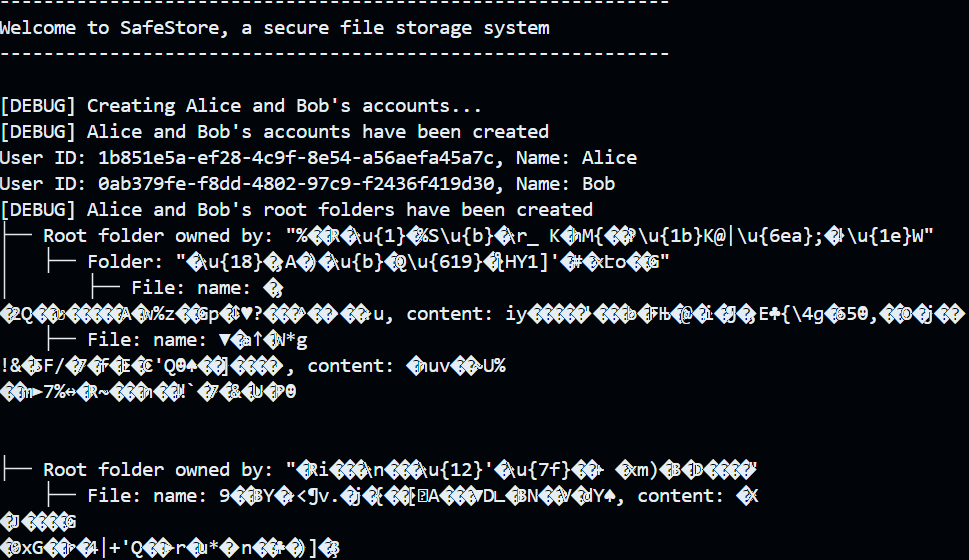
\includegraphics[width=\textwidth]{screenshots/create_procedure.png}
    \caption{Account creation procedure}
    \label{fig:create_procedure}
\end{figure}

It is important to note that the server's contents are all encrypted and this is why we see these bizarre character chains in \autoref{fig:create_procedure}. We are trying to print encrypted data to the console.


\subsubsection{Login procedure}
To decrypt the root folders we must first login as Alice. We can then decrypt her root folder:

\begin{figure}[H]
    \centering
    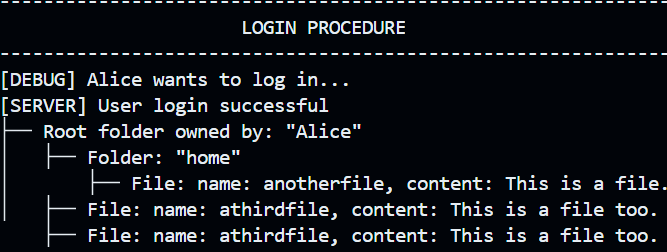
\includegraphics[width=\textwidth]{screenshots/login_procedure.png}
    \caption{Login procedure}
    \label{fig:login_procedure}
\end{figure}

As we can see in \autoref{fig:login_procedure}, Alice's root folder was decrypted. This happens client side so the server will not get any information.

\subsubsection{Password change procedure}
Alice is now logged in and she may change her password. To do this she first creates a new password, calculates a new corresponding password hash and challenge hash. She gives the challenge hash and the new password salt to the server for safekeeping. In addition to the new values, she \textbf{must} provide the same "old" challenge hash she used to login because the logout procedure with password change will perform a similar authenticity process as the login procedure. If it didn't perform this check, someone could potentially change her password without her being logged in. It automatically checks at each logout if those values are present. If they are, it updates its lists.

\begin{figure}[H]
    \centering
    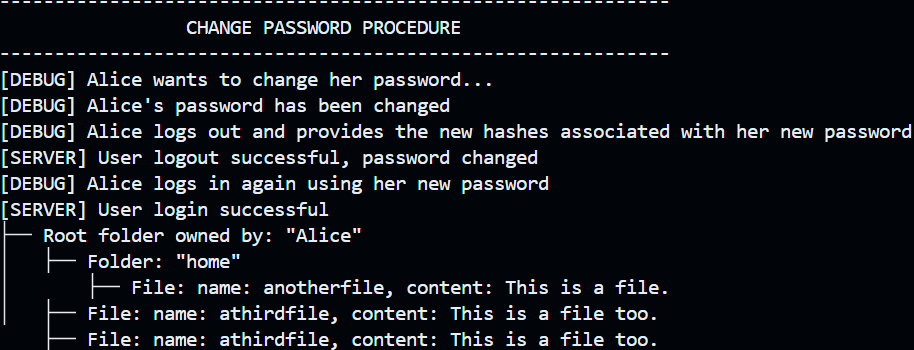
\includegraphics[width=\textwidth]{screenshots/password_procedure.png}
    \caption{Change password procedure}
    \label{fig:password_procedure}
\end{figure}

Again, all of the decryption and encryption with the new password happens client-side. The server never gets any additional information except for the new challenge hash and password salt. But alone, these are useless.

\subsubsection{Sharing folder procedure}
Alice wishes to share her "home" folder with Bob. For this, she uses Bob's public key and asymmetrically encrypts it. She then signs the hole folder. Bob receives the encrypted folder, he can verify its signature with Alice's public key as to ensure integrity of the contents. He may then decrypt it with his private key. He can then do some work on the folder.

\begin{figure}[H]
    \centering
    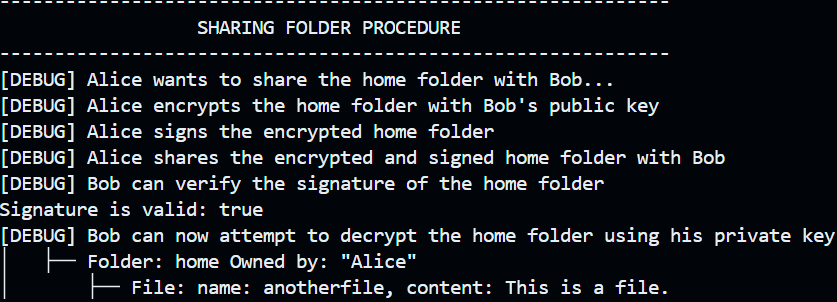
\includegraphics[width=\textwidth]{screenshots/share_procedure.png}
    \caption{Sharing folder procedure}
    \label{fig:share_procedure}
\end{figure}




